\subsection{Chargers}\label{sec:chargers}
\subsubsection{Controlling the chargers}
One of the main functionalities of the ODROID is to turn on the chargers if a user wants to charge an e-bike \ref{eis:1.6}. Turning on the chargers is done using a relais that is controlled by the ODROID. The relais can be turned on or off by using a signal from a GPIO pin.\\

At this moment the physical chargers that will be used in the charging station are not developed enough to be used for test purposes, hence another way to test the C-code must be designed. An easy way to check if the GPIO pins are turning the chargers on or off is by using LEDs that are connected to the GPIO pins. However, it is not desired to draw current for the LEDs directly from the GPIO pins. Since the driving current limit for the GPIO pins is 2-4 mA (not every pin has the same current limit) \cite{odroid_currentlimit}, it is neccesary to use an external driver for the LEDs. The easiest way of driving a LED is by using a voltage controlled switch. The voltage from the GPIO pins then determines whether the switch is open or closed. In electronic components, such a voltage controlled switch can be made by using a transistor \cite{switch_transistor}. To behave as a closed switch the transistor must be in saturation, because then the collector to emitter resistance is very low and the transistor almost acts as a short circuit. For the transistor to behave as an open switch, it must be in cutoff mode.\\

\begin{figure}[!ht]
  \centering
    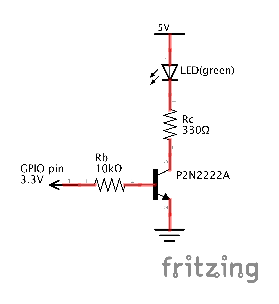
\includegraphics[scale=1.5]{images/led_driver_schem.pdf}
      \caption{Circuit used to drive the LED. Made using Fritzing \cite{fritzing}}\label{fig:leddriver}
\end{figure}

The transistor used for this circuit is a bipolar P2N2222A NPN transistor. This is a general purpose transistor that can be used for power amplification as well as switching applications requiring collector currents up to 500mA \cite{p2n2222a}.\\

\Cref{fig:leddriver} shows the circuit that is used. Resistor Rc is chosen such that the current through the LED is limited if the LED turns on, hence a maximum current of $\frac{5}{330}=15mA$ can be drawn from the source. However, since there is also a voltage drop over the LED this current will be much smaller and well below the current limit for this LED.\\

In order to act as a buffer, the circuit should draw as less current as possible from the GPIO pins of the ODROID. This is achieved by choosing a very high base resistance Rb. However, a base resistance that is too high results in malfunctioning of the transistor because not enough current is fed into the base. 

When the transistor is in saturation the base voltage is about 0.7V thus the base current is about $\frac{3.3-0.7}{Rb}$. To achieve a base current of 0.1mA a resistance Rb of 26k$\Omega$ is needed. However, after a test this resistance was found out to be too large. A smaller resistor of 10k$\Omega$ solved this problem.\\

The circuit shown in \Cref{fig:leddriver} is built six times and then connected to the six GPIO pins of the ODROID that are used to control the chargers \ref{eis:3.4}.\\

\subsubsection{Detection of the charging cable}
To increase the level of safety for the users the chargers should not be turned on when there is nothing connected to them. Therefore a charging cable detection system is designed. For each cable one additional GPIO pin is needed (of course the ground pin on the ODROID is also needed). In case of a connected charging cable, this GPIO pin is shorted to ground (inside the charging cable) and thus a logic 0 is set to this pin. In the other case (no connected charging cable), the pins keep floating. However, the ODROID can be programmed such that it internally connects a pull-up resistor to the pin. Now a logic 1 is detected whenever no charging cable is detected. Within the C-code this can be detected by using the \verb|digitalRead()| and \verb|pullUpDnControl()| functions.\\

\begin{figure}[!ht]
  \centering
    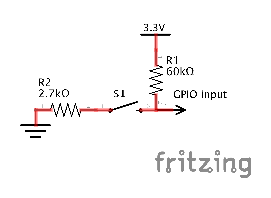
\includegraphics[scale=1.7]{images/cable_detection_schem.pdf}
      \caption{Circuit used to detect the connected cable using a GPIO pin \cite{fritzing}}\label{fig:cable_detect}
\end{figure}

\Cref{fig:cable_detect} depicts the circuit that is used for this purpose. Since there are no available charging cables yet, a switch was used in this circuit to simulate the behaviour of the cable. It was also chosen to include a 2.7k$\Omega$ resistor in series with the switch. As a testing circuit some precautions have to be taken to ensure that nothing can be damaged as a result of short circuits. This also results in a choice for the value of resistor R2. The lowest current limit of all GPIO pins is 2mA. Together with a maximum voltage of 5V on one of the pins, a 2mA current limit means that R2 must be at least 2.5k$\Omega$.\\

But R2 may limit the short circuit current, it also influences the voltage at the pin. The voltage division on R1 and R2 makes that it is no longer possible to obtain 0V at the GPIO pin. With the switch in closed state, the voltage is $\frac{R2}{R1+R2}\cdot 3.3 = \frac{2.7}{62.7}\cdot 3.3=0.14V$. Altough this voltage is not zero, it is nevertheless low enough for the ODROID to detect it as a logic low or 0. With the switch in opened state, this voltage division does not occur and will thus not impose problems with respect to the input voltage.\\

\subsubsection{Control mechanism for the chargers}\label{sec:charger_control}
When a reservation is made in the end-user interface the state of the charger in the database is set to 1. Using the C-code on the ODROID this data can be retrieved from the server. When calling the function \verb|getChargerState()| an array of length 6 is returned, containing the server state of all chargers. As explained in \Cref{sec:code_overview} the chargers are set every 1.5 seconds using the function \verb|setChargers()|.\\ 

For the design of this control mechanism some additional functionalities were set up to improve user-friendliness and safety. These are:
\begin{itemize}
\item When a reservation is made on the website, but the owner of the e-bike does not show up within 60 seconds, the charging point is released. This ensures that it is not possible to claim charging points without actually charging.
\item The chargers will only be switched on when a cable is connected for more than 6 seconds.
\item In case of a cable that is being disconnected during charging, the chargers will turn off, but remain reserved for 15 seconds. A cable that is plugged out accidentally can now be replaced without having to login again.
\item The admin-dashboard must be able to turn off a charger, even when a vehicle is connected.\\
\end{itemize}

\begin{figure}[!ht]
  \centering
    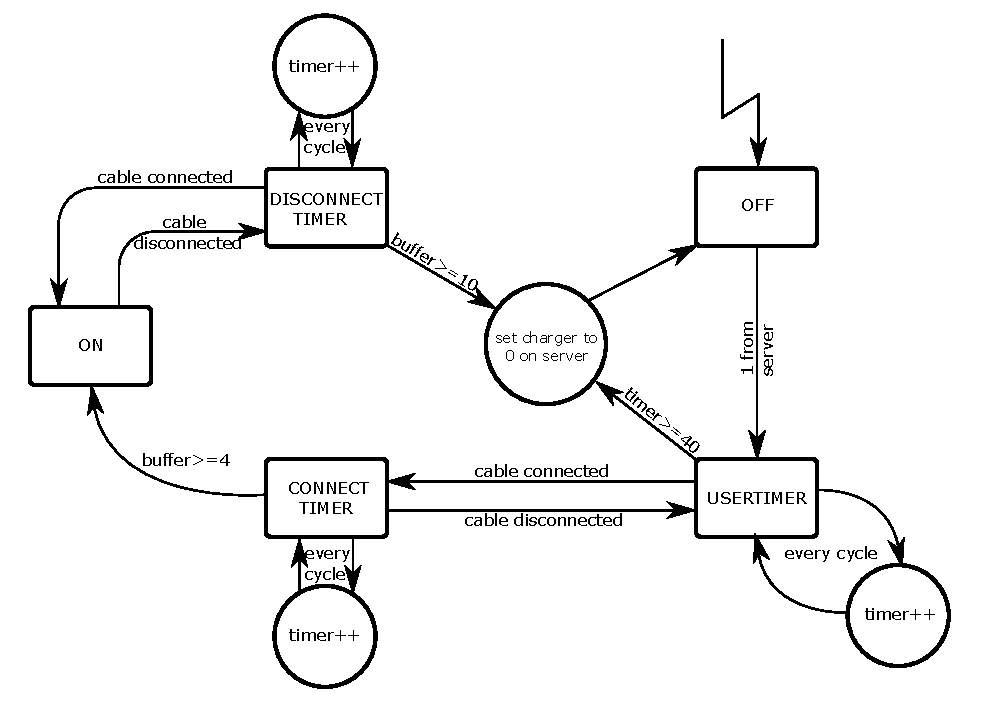
\includegraphics[width=\textwidth]{images/Charger_Control.pdf}
      \caption{FSM to control the chargers}\label{fig:fsm}
\end{figure}

To implement these functionalities, it can be seen that three different timers are needed and thus some form of memory to store these timers. Moreover, the chargers must refresh or reset every time the variable \verb|j| from \Cref{fig:code_overview} is incremented (every 1.5s). All these functionalities can now conveniently be combined in a Finite State Machine (FSM) that uses a change in \verb|j| as the clock. \Cref{fig:fsm} depicts the finite state machnine that was designed for this purpose.\\

The diagram starts in the reset state, which is the OFF state. It only leaves this state when a reservation is made and the server says that a charger must be turned on. In that case the finite state machine goes into the USERTIMER state. Here it waits until a cable is connected. When no charging cable is connected within 60 seconds, the FSM goes back to the OFF state and sends a message to the server that the charger can be freed for other users. In the other case (charging cable is connected within 60 seconds), the FSM goes to the CONNECTTIMER state. Here it waits 6 seconds until it moves on to the ON state where the chargers are switched on. However, if the cable is disconnected within these 6 seconds, the FSM returns to the USERTIMER state. Now the cable must be plugged in for another 6 seconds before the chargers are switched on.\\

Now suppose the e-bike is being charged and the finite state machine is in the ON state and the charging cable is disconnected. This can be due to two reasons: the e-bike is charged and leaves, or the e-bike is accidentally unplugged. Both cases will make the FSM move to the DISCONNECTTIMER state where the charger is turned off. If the cable is reconnected within 15 seconds, the FSM moves back to the ON state and the charger is turned back on again. On the other hand, after 15 seconds of no reconnection, the charger is left off and the FSM moves to the OFF state.\\

Finally, if the FSM moves to a next state, the timer of the corresponding state that is left, is reset. All three timers are reset when a charger is turned off on the admin-dashboard. The FSM then always moves to the OFF state.\\

To obtain a Moore machine, the output signals must only depend on the current state. Hence the chargers are turned on only in the ON state, whereas in all other states, the chargers are off. Using the C library \textit{WiringPi} \cite{WiringPi} it is possible to easily write a logic 0 or 1 to the GPIO pins and effectively turn the chargers on or off \cite{wiringpi_functions}. The GPIO \textit{WiringPi} pin numbers used for this purpose are 6, 10, 11, 12, 13 and 14 for the chargers and 21, 22, 23, 24, 26 and 27 for the cable detection \cite{odroid_specs}. Each of the six chargers is controlled by an FSM and hence 6 FSMs are neccessary to control all chargers. It is chosen to implement this by using a \verb|for|-loop.

\subsubsection{Internet failure failsafe}
A failsafe was implemented which ensures that e-bikes are not connected for too long when internet is unavailable. This is important because the station cannot be monitored online during an internet outage. A timer was made that keeps track of how long the internet has been down for. It was decided that all chargers should be turned off whenever the internet is out for more than 2 hours. This time was chosen because it enables the station to finish the charging of any e-bike that is already connected, while also limiting potential risks of an unmonitored system.\\

\scriptsize
	\lstinputlisting [language=C,caption=Internet failure failsafe,label=script:internet_failure_failsafe] {code/internet_failure_failsafe.c}
\normalsize

The implementation of this failsafe can be found in Script \ref{script:internet_failure_failsafe}. In this function, the first \verb|if| statement checks if the data fetch was successful. In this statement, the \verb|noConnectionTimer| is set to zero. The \verb|else|-statement is executed whenever connection was not successful. In this part, the \verb|noConnectionTimer| is incremented (or set to one if the system just booted with no connection). The timer value is then checked if it is larger than $2\cdot60\cdot60/1.5=4800$ (one poll every 1.5 seconds), and the GPIO pins are set to low if it is. Note that the \verb|for|-statements in the case of no connection manage the charger GPIOs and the FSM states as described in \Cref{sec:charger_control} (omitted for the sake of simplicity).